\section{Design patterns}
\enumstart
	\item Motivation
	\enumstart
		\item Designing object-oriented software isn't trivial
		\enumstart
			\item Create classes at the right granularity
			\item Establish inheritance hierarchies
			\item Establish relationships between classes
			\item Define interfaces
		\enumend
		\item Good design
		\enumstart
			\item Solves the current problem
			\item Is general enough for future requirements
		\enumend
		\item You're not the first one to write software
		\item Goal: Reuse solutions that worked in the past
		\item Design patterns: Reusable solution to a commonly occuring problem in software design
	\enumend
\enumend

\subsection{Composite pattern}
\enumstart
	\item A program manipulates
	\enumstart
		\item individual objects
		\item Compositions of objects that form a part-whole hierarchy
	\enumend
	\item Want to allow algorithms to treat individual objects and compositions of objects uniformly
	\\ 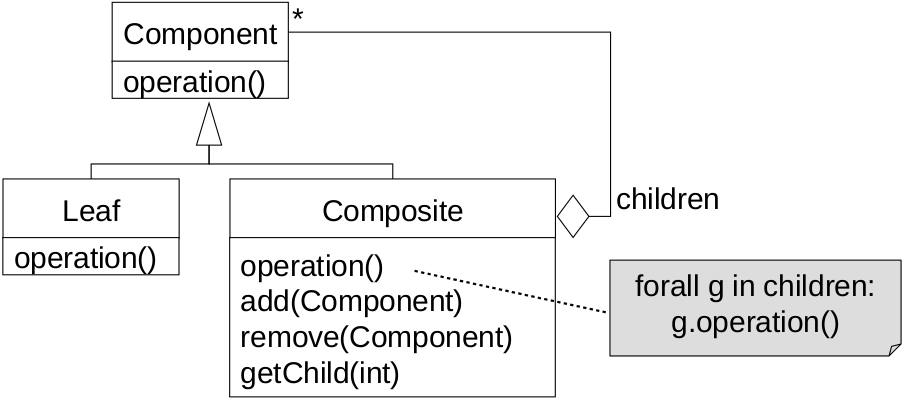
\includegraphics[width=0.5\textwidth]{img/composite_pattern.png}
	\item Properties
	\enumstart
		\item Makes clients simple: Composite objects used like primitive objects
		\item Easy to add new kinds of objects
		\item Can make the design too general
	\enumend
	\item Implementation
	\enumstart
		\item Explicit parent references
		\item Sharing components - reduces memory requirements (flyweight-pattern)
		\item Order of children
		\item Caching to improve performance
		\item Data structure for storing components
	\enumend
\enumend

\subsection{Object adapter pattern}
\enumstart
	\item Problem: incompatible interfaces
	\\ 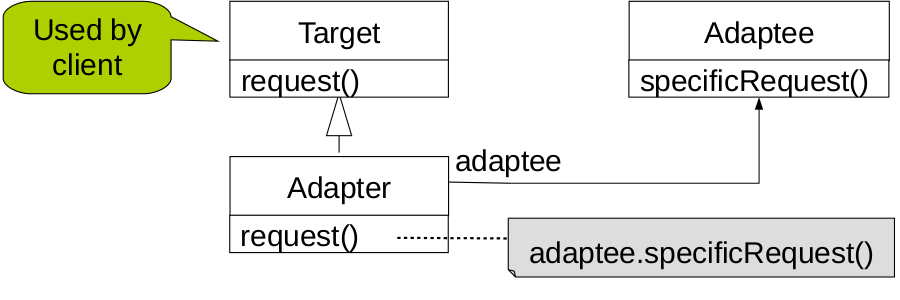
\includegraphics[width=0.5\textwidth]{img/object_adapter_pattern.png}
	\item Structure
	\enumstart
		\item Adapter forwards to adaptee
		\item Subtyping used to specify interface to adapter
		\item Target and adaptee exist before adapter
		\item Target may be an interface in Java
	\enumend
	\item Properties
	\enumstart
		\item Can adapt multiple existing subclasses without subclassing each of them
		 \item Ovelleo.orgrride adaptee's behaviour is harder, because of object schizophrenia
	\enumend
\enumend

\subsubsection{Object schizophrenia}
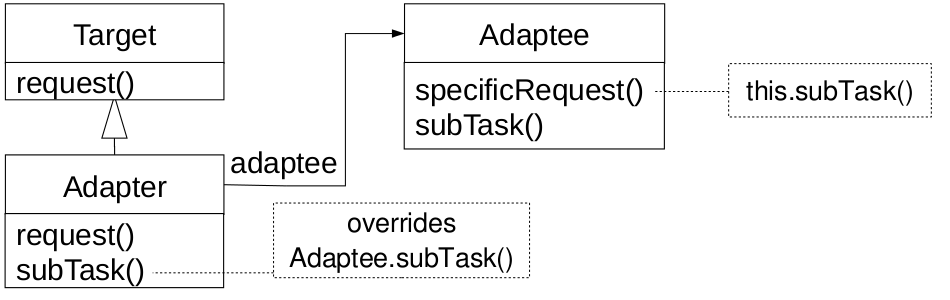
\includegraphics[width=0.5\textwidth]{img/object_schizophrenia.png}
\enumstart
	\item Forwarding request() to specificRequest() will not lead to a call to Adapter.subTask()
	\item Problem: Two objects represent one conceptual object
\enumend

\subsection{Class adapter pattern}
\enumstart
	\item Alternative to object adapter
	\\ 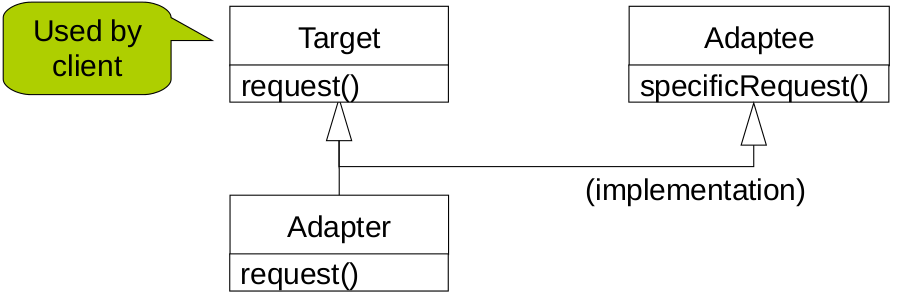
\includegraphics[width=0.5\textwidth]{img/class_adapter_pattern.png}
	\item Structure
	\enumstart
		\item Adapter inherits implementation from adaptee
		\item Target and adaptee exist before adapter
		\item Target must be an interface in Java
	\enumend
	\item Properties
	\enumstart
		\item Adapts one class at a time
		\item Can override some of adaptees behaviour
		\item Only one object, no indirection
	\enumend
\enumend

\subsection{Abstract factory pattern}
\enumstart
	\item Problem: create objects without knowing their concrete class
	\\ 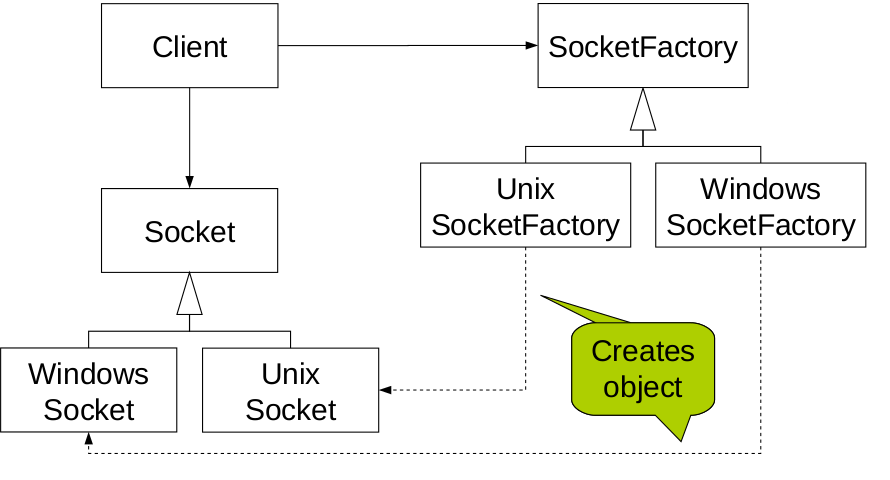
\includegraphics[width=0.5\textwidth]{img/abstract_factory_pattern.png}
	\item Applicability
	\enumstart
		\item System should be independant of how its classes are created, composed and represented
		\item Multiple families of related classes - Must decide on one family
		\item Provide a library of classes and reveal only their interfaces, not their implementations
	\enumend
	\item Properties
	\enumstart
		\item Isolates concrete classes
		\enumstart
			\item Helps control what classes are instantiated
			\item Isolates classes from implementation classes
		\enumend
		\item Exchanging product families is easy
		\enumstart
			\item Concrete factory appears only once in a program
		\enumend
		\item Supporting new kinds of products is difficult
		\enumstart
			\item Affects interface of abstract factory and all concrete factories
		\enumend
	\enumend
\enumend

\subsection{Singleton pattern}
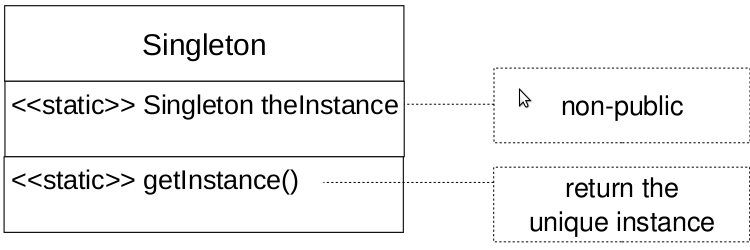
\includegraphics[width=0.5\textwidth]{img/singleton_pattern.png}
\enumstart
	\item Exactly one instance of a class
	\item Generalizable to any number of instances
	\item Sometimes part of the programming-language
	\item Applicability
	\enumstart
		\item Ensure that a class has only one instance and provide a global point of access to it
		\item A global variable alone is insufficient - May still have multiple instances
	\enumend
\enumend

\subsection{Iterator pattern}
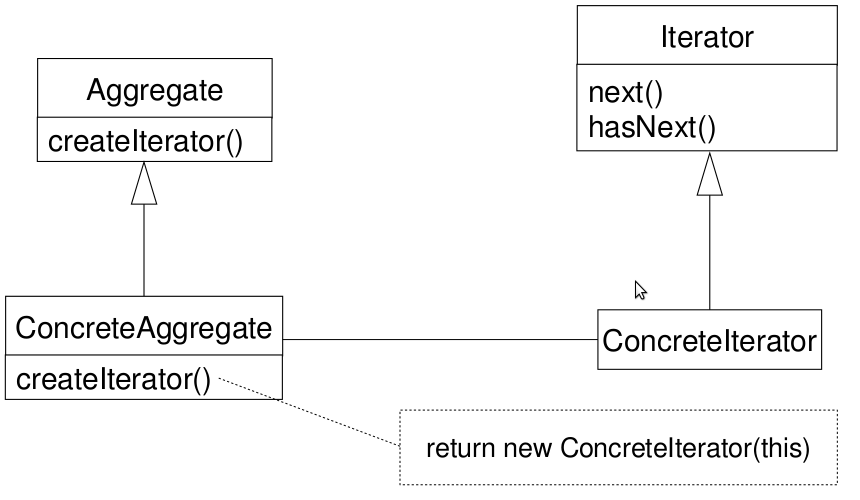
\includegraphics[width=0.5\textwidth]{img/iterator_pattern.png}
\enumstart
	\item Applicability
	\enumstart
		\item Provides a way to access the elements of a container without exposing it's internals
		\item Support multiple traversals of aggregate objects
		\item Provide a uniform interface for traversing different kinds of aggregate structures
	\enumend
	\item Properties
	\enumstart
		\item Separate implementation of traversals from implementation of aggregate object
		\item Simplifies the aggregates interface - Can support different kinds of traversals with a single method iterator()
		\item Easy to switch between variations of traversal
	\enumend
\enumend

\subsection{Observer pattern}
\enumstart
	\item Problem: Maintain Consistency between loosely coupled objects
	\\ 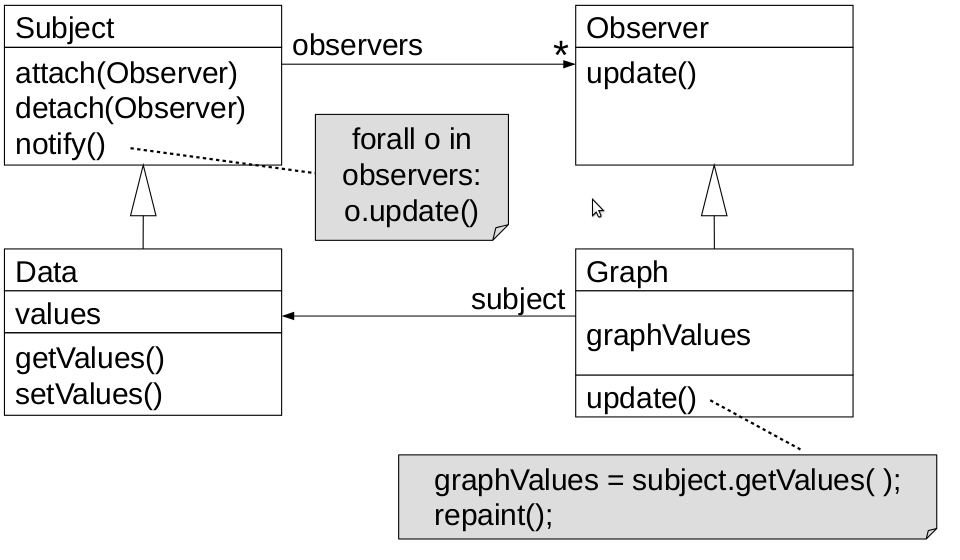
\includegraphics[width=0.5\textwidth]{img/observer_pattern.png}
	\item Applicability
	\enumstart
		\item Many dependant objects must be informed, when one object (subject) changes its state
		\item Subject should not depend on its dependants
	\enumend
	\item Properties
	\enumstart
		\item Loose coupling - alows layering
		\item Support for broadcast communication - add/remove observers dynamically
		\item Also known as: Listener, Publish-Subscribe
	\enumend
\enumend

\subsection{Strategy pattern}
\enumstart
	\item Problem: Exchangeable algorithms
	\\ 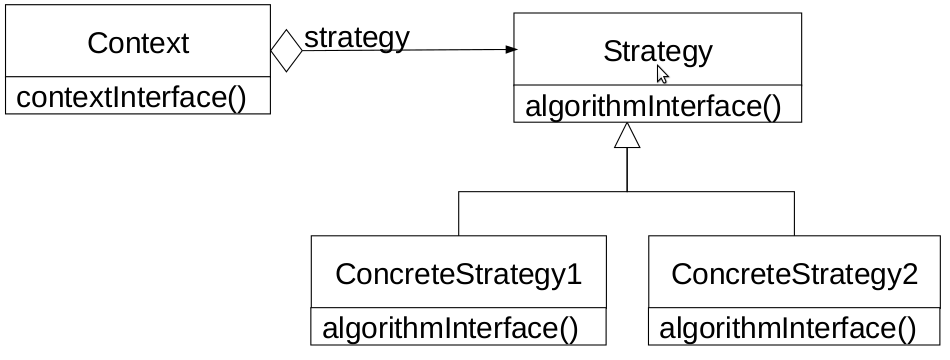
\includegraphics[width=0.5\textwidth]{img/strategy_pattern.png}
	\item Applicability
	\enumstart
		\item An algorithm has different variations, each appropriate for a different situation
		\item Want to vary the algorithm without changing the client
		\item Algorithms are complex and should be encapsulated in their own classes
	\enumend
	\item Properties
	\enumstart
		\item Supports families of algorithms
		\item Alternative to inheritance
		\enumstart
			\item Behaviour not hardwired but dynamically exchangeable
			\item Seperates context from algorithm - easier to maintain
		\enumend
		\item Communication overhead - Must pass all required data to algorithm
	\enumend
\enumend

\subsection{Template method pattern}
\enumstart
	\item Problem: Refinement of algorithms
	\\ 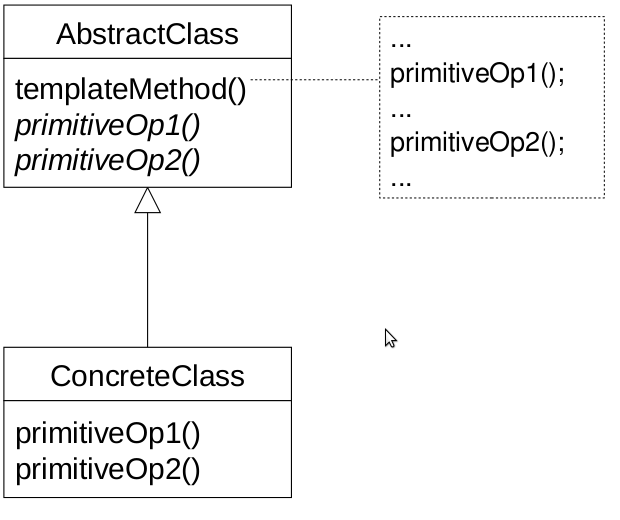
\includegraphics[width=0.5\textwidth]{img/template_method_pattern.png}
	\item Applicability
	\enumstart
		\item Want to refine steps of an algorithm without changing its overall structure
		\item An algorithm has several variant and an invariant part
		\item Want to avoid code duplication of the invariant part
	\enumend
	\item Properties
	\enumstart
		\item Inverted call-structure - Parent calls child, not the other way around
		\item Abstract class may define defaults for some primitive operations
		\item Primitive operations are often non-public
	\enumend
\enumend

\subsection{Visitor pattern}
\enumstart
	\item Problem: Operate on an object structure
	\\ 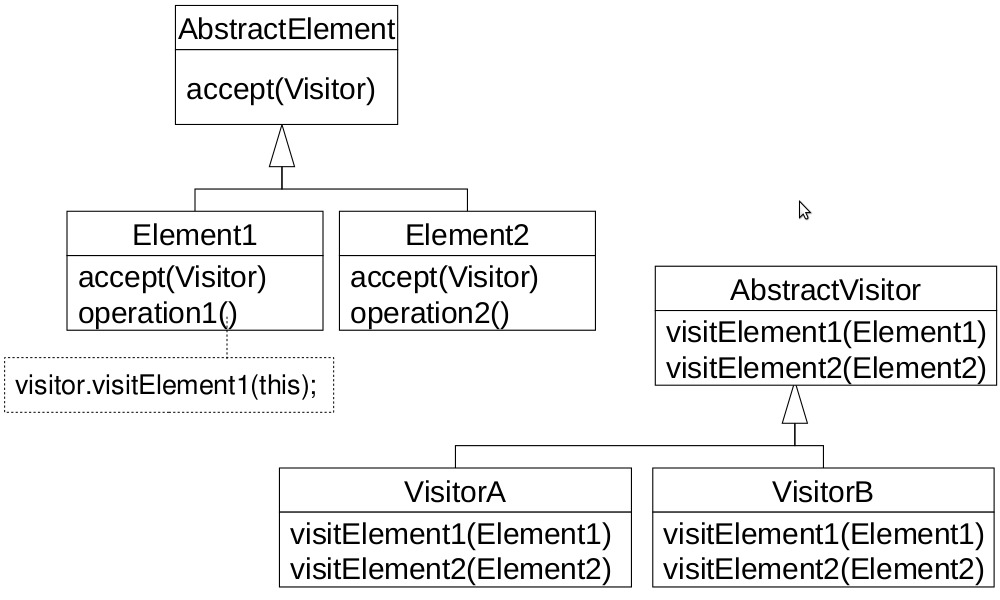
\includegraphics[width=0.5\textwidth]{img/visitor_pattern.png}
	\item Applicability
	\enumstart
		\item Object structure with many classes
		\item Many operations to be performed
		\item Operations depend on concrete class of object
		\item Classes of object structure rarely change
	\enumend
	\item Properties
	\enumstart
		\item Changing/adding operations is easy - each operations encapsulated in one class
		\item Changing the object structure is difficult - must adapt all visitors
		\item implements double dispatch in a language with single dispatch
	\enumend
\enumend

\subsubsection{Double dispatch}
\enumstart
	\item Objects have a static and a dynamic type
	\item Dynamic dispatch - choose method based on dynamic types
	\item Often: Single dispatch on method receiver
	\item Sometimes needed: Double dispatch on receiver and arguments
\enumend

\subsection{Facade pattern}
\enumstart
	\item Problem: Unified interface for a subsystem
	\\ 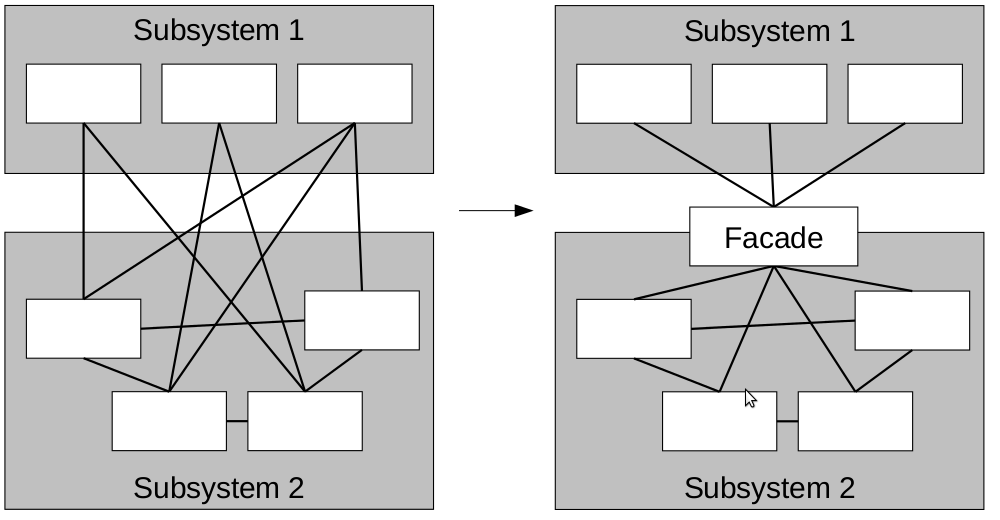
\includegraphics[width=0.5\textwidth]{img/facade_pattern.png}
	\item Properties
	\enumstart
		\item Highlevel interface that makes subsystem easier to use
		\item Reduces coupling
		\item Most of the time, facade need not to be changed when subsystem changes
		\item Does not prevent direct usage of objects within a subsystem
	\enumend
\enumend

\subsection{Command pattern}
\enumstart
	\item Problem: Encapsulate actions
	\\ 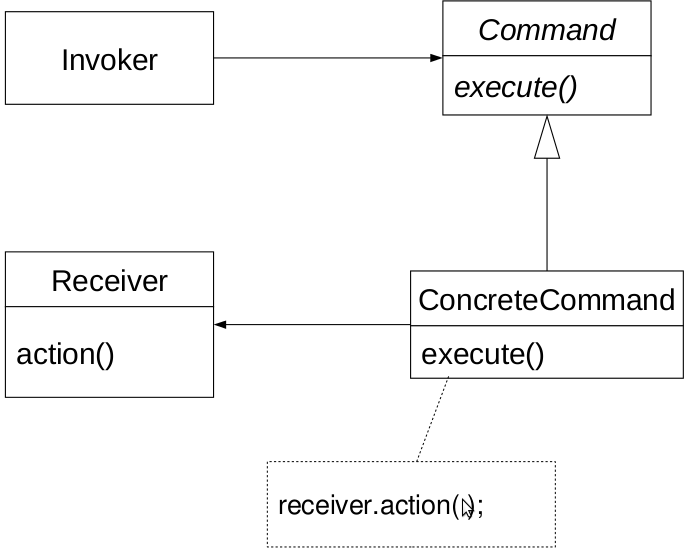
\includegraphics[width=0.5\textwidth]{img/command_pattern.png}
	\item Applicability
	\enumstart
		\item Actions to be performed should be first class entities
		\item Specify, queue, and execute requests at different times
		\item Support undo/redo
	\enumend
	\item Properties
	\enumstart
		\item Decouples the object that invokes an operation from the one that knows how to perform it
		\item Commands can be extended and manipulated like any other object
		\item Can assemble commands into macro commands
		\item Adding new commands is easy - no need to change other classes
	\enumend
\enumend

\subsection{Bridge pattern}
\enumstart
	\item Problem: Vary abstraction and implementation independantly
	\\ 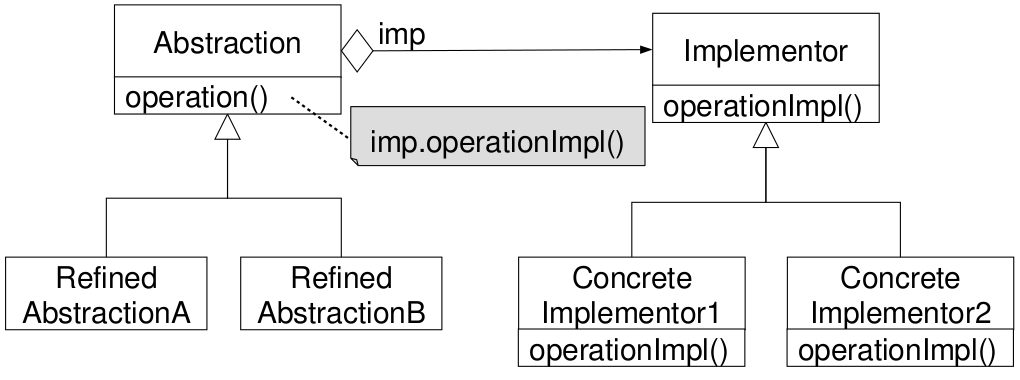
\includegraphics[width=0.5\textwidth]{img/bridge_pattern.png}
	\item Applicability
	\enumstart
		\item Have two dimensions that vary independantly
		\item Want to avoid explosion of class hierarchy
		\item Changes in implementation should not affect clients
	\enumend
	\item Properties
	\enumstart
		\item Implementations of an interface can be exchanged dynamically
		\item Can extend abstraction and implementation hierarchy independantly
		\item Hides implementation details from client
	\enumend
	\item Bridge vs. Adapter
	\enumstart
		\item Both used to hide details of underlying implementation
		\item Adapter
		\enumstart
			\item Makes unrelated components work together
			\item Applied after a system is designed
		\enumend
		\item Bridge
		\enumstart
			\item Used up-front to design an extensible system
		\enumend
	\enumend
\enumend
